\chapter{Evaluation}

In this section, we present the evaluation of our IT artefact, aimed at addressing the two research questions.
The evaluation study focuses on two key dimensions. 
Firstly, we examine the effectiveness of the system in enhancing users' comprehension of the recommended energy technologies and their advantages. 
Secondly, we gauge the level of trust that users place in the recommendations provided by the system. 
Additionally, we seek to explore whether the information presented influences users' perspectives and behaviours, 
encompassing aspects such as their familiarity with energy-efficient technologies and their inclination to adopt them. 

As highlighted in Nunes and Jannach's summary \cite{Nunes2020}, 
there is no universally accepted definition of what constitutes a correct or best explanation, 
evaluating the quality of explanations relies on capturing the subjective perceptions of users and monitoring the impact of these explanations on user behaviour, 
and user studies have been the predominant research method for assessing explanations in recommender systems.
Aligned with this understanding, our goal of capturing the subjective perceptions of users regarding the explanations provided and their attitude changes, 
we have made the decision to conduct real-user studies. 

Due to time constraints imposed by the university's requirements for a master's thesis, we conducted qualitative user studies with \textcolor{cyan}{7} participants in \textcolor{cyan}{Germany}. 
While the sample size was small, qualitative studies provide valuable insights into rusers' perceptions, attitudes, and experiences.


\subsubsection{Goals}

The evaluation aims to achieve two primary objectives, to understand: 
\begin{itemize}
  \item Efficacy in addressing the information gap.
  \item Level of trust towards the recommendations.
\end{itemize}


\section{Semi-structured interviews}

The interview proceeds through the following steps.
\begin{enumerate}
  \item Express gratitude to the interviewee for their willingness to participate and introduce myself briefly.
  \item Provide a brief recap of the project, emphasising its purposes, and clarify the specific objectives of the interview.
  \item Inform the interviewee about the expected duration of the interview and assure them that the recording will be used solely for transcription purposes, ensuring confidentiality.
  \item Explain that the interview will involve participants using the web service to explore and discover recommendations tailored to their home situations.
  \item Prior to participants using the service, they will be asked a series of questions pertaining to their demographic information and initial perceptions of energy technologies.
  \item Ask participants to use the service using a laptop and encourage them to think-out-loud while navigating.
  \item When the participants finished interacting with the service, other questions will be asked.
  \item Inquire if the interviewee has any remaining questions or uncertainties.
  \item Express appreciation once again for their participation and inform them that they can reach out with any further concerns or inquiries they may have.
\end{enumerate}


\subsubsection{Target groups}

The target users of this study are individuals residing in Germany who own or live in single-family houses.
The participants were recruited using a convenient sampling approach. 
We employed a snowball technique by reaching out to acquaintances to inquire about their residence in a single-family house or their knowledge of individuals residing in such properties. 

The interview invitation is composed as follows:

\textbf{Are you a homeowner in Germany with a single-family house? 
Do you want to make informed investment decisions about energy technologies for your home? }
If so, we invite you to participate in a 1-hour interview for our web service developed in collaboration with the University of Siegen.
Don't miss out on the opportunity to finding out some energy technologies to invest for your home that potentially save energy cost. 
During the interview, you will use our online service and share your experience.
Rest assured that all information shared will be kept confidential and anonymised. 
The interview will be conducted either remotely or in person as you prefer. 
If you are interested, please choose your preferred time slot by clicking on the following link: https://calendar.app.google/F8RnWSKmnofz3cHf6. 
If you have any questions, feel free to contact us.
Thank you for considering collaborating on the project! 

Every participant took part in the evaluation signed a consent form (Appendix \ref{appendix:consentform}) before starting. 
A summary of the participants can be found in Table \ref{tab:participants}.
\begin{table}[h!]
  \centering
  \begin{tabular}{ | p{.10\textwidth} | p{.10\textwidth} | p{.10\textwidth} | p{.20\textwidth} | p{.20\textwidth} | } 
    \hline
    ID & Gender & Age & Nationality & Occupation \\
    \hline
    PA & M & 60 & Germany & Constructor \\
    \hline
    PB & M & 30 & Germany & Researcher \\
    \hline
    PC & F & 28 & Taiwan & HCI student \\
    \hline
    PD & F & 69 & Germany & Retired professors \\
    \hline
    PE & M & 69 & Germany & Retired professors \\
    \hline
    PF & M & 29 & Austria & PhD student \\
    \hline
    PG & M & 28 & Germany & PhD student \\
    \hline
  \end{tabular}
  \caption{Participants}
  \label{tab:participants}
\end{table}


\subsubsection{Material}

\begin{itemize}
  \item \textbf{Laptop:} Participants will be provided with a laptop to access and use the web service before the interview. 
  \item \textbf{Recording Device:} A mobile phone for instance, will be used to capture and record the interview session to enable accurate transcription of the interview responses for analysis and reference.
  \item \textbf{Interview Guideline:} A printed copy of the interview guideline.
  \item \textbf{Pen and Papers:} A pen and some papers to jot down any notes or additional information during the session. 
  \item \textbf{Translator:} In the event that participants are not comfortable with the English language, a German speaker will be present to assist in facilitating communication and ensuring a clear understanding of the questions and responses.
\end{itemize}


\subsubsection{Welcome}

Thank you for participating in this interview. 
My name is Yanwei Miao, and I am currently working on my master's thesis project in collaboration with Fraunhofer ISI.
We developed a web service to help homeowners like you make informed decisions about investing in energy technologies for your homes. 
Our aim is to provide personalised recommendations based on your specific circumstances, enabling you to determine the economic feasibility of implementing these technologies. 
To proceed, we kindly request your cooperation in answering a few questions about your background. 
This will help us gain a better understanding of your knowledge and perspective on AI and energy technologies. 
Once is complete, we will guide you through the web service to obtain personalised recommendations for your home energy system. 
While using the service, we encourage you to think out loud and share your thoughts and observations. 
Afterward, we will conduct an interview to gather your feedback and insights. 
If you have any questions at any point, please don't hesitate to ask. 
Are you ready to begin?


\subsubsection{Questions}

The interview questions can be categorised into four main categories: \emph{demography, knowledge, trust, and additional questions}.
Demography questions focus on gathering information about the background of the interviewees, aiming to identify any demographic factors that may influence their interest in more detailed explanations.
Explainability questions are designed to assess the clarity and comprehensibility of the provided explanations, aiming to determine if they are clear and understandable to the participants. 
Attitude change questions are divided into two parts: before using the service and after using the service. 
These questions aim to capture any changes in participants' attitudes towards energy technologies and their perception of the recommendations after using the service.
Lastly, additional questions or thoughts may arise during the interview. 
They could be an opportunity to explore additional insights or address any specific concerns during the conversation. 

\begin{center}
  \small
  \begin{longtable}{ | p{.20\textwidth} | p{.70\textwidth} | }
    \hline
    \textbf{Category} & \textbf{Questions} \\
    \hline
    \multicolumn{2}{|l|}{\cellcolor{lightgray}Before using the web service} \\
    \hline
    \multirow{6}{4em}{Demography} & Gender \\
    & Age \\
    & Educational background \\
    & Occupation \\
    & Nationality \\
    & Knowledge and interest in AI \\
    & Knowledge and interest in the energy domain \\
    \hline
    \multirow{4}{4em}{Knowledge} & Have you heard of energy-efficient appliances or renewable energy technologies for households? \\
    & Have you ever considered implementing energy-efficient technologies, such as solar panels and smart thermostats in your house? \\
    & What is your understanding regarding the benefits of energy-efficient technologies? \\
    & Do you know climate change and why it is important for individuals to save energy and utilise renewable energy sources? \\
    \hline
    \multicolumn{2}{|l|}{\cellcolor{lightgray}After using the web service} \\
    \hline
    \multirow{7}{4em}{Trust} & How do you feel about the recommendations provided? \\
    & Do you find the recommendations useful or valuable? \\
    & Are you considering investing in any of the recommended technologies now? Why or why not? \\
    & What factors influence your decision to adopt or reject the recommendations? \\
    & Do you know why the recommendations were recommended to you? \\
    & Do you trust the recommendations? Why or why not? \\
    & What factors contribute to your trust or lack of trust in the recommendations? \\
    \hline
    \multirow{4}{4em}{Knowledge} & Were you familiar with these technologies before using the system? \\
    & Did the system provide enough information for you to understand the technologies? \\
    & Has your knowledge of energy efficient technologies improved as a result of using the system? \\
    & Do you believe adopting these technologies can lead to lower energy costs? Why or why not? \\
    \hline
    \multirow{2}{4em}{Additionals} & Give participants an opportunity to share any additional thoughts, concerns, or suggestions regarding the system and its recommendations. \\
    & Ask if they have any questions for you or if there's anything else they would like to discuss. \\
    \hline
  \caption{Interview guideline}
  \label{tab:interview}
  \end{longtable}
\end{center}


\subsubsection{Closure}

Thank you so much for taking the time to participate in this interview session. 
I sincerely appreciate your willingness to share your thoughts and experiences with us. 
If you have any further questions, concerns, or additional insights that you would like to share, please don't hesitate to reach out. 


\section{Future work: Kano survey}

The Kano model \cite{Sauerwein1996} is a commonly used framework in quantitative research to understand customer satisfaction and prioritise features or attributes. 
In our project, we aim to also incorporate the Kano model survey (Table \ref{tab:kanomodel}) as part of our future work. 
We plan to integrate this survey directly into the web service, allowing individuals who have interacted with the service online to voluntarily complete the survey.
Through the integration of the Kano survey into the web service, we have the opportunity to collect insights from users who engage with the service online. 
This will enable us to assess whether the inclusion of specific features in the service brings delight to our users.
This assessment will help us determine the necessity of explanations in the service as well. 

\begin{center}
  \small
  \begin{longtable}{ | p{.40\textwidth} | p{.06\textwidth} | p{.06\textwidth} | p{.06\textwidth} | p{.06\textwidth} | p{.06\textwidth} |}
    \hline
    Features & I like it & I expect it & I'm neutrual & I can tolerate it & I dislike it \\
    \hline
    Show corresponding yearly energy bill &&&&& \\
    \hline
    Don't show corresponding yearly energy bill &&&&& \\
    \hline
    Show detailed simulated yearly energy consumption &&&&& \\
    \hline
    Don't show detailed simulated yearly energy consumption &&&&& \\
    \hline
    Show detailed simulated daily energy consumption &&&&& \\
    \hline
    Don't show detailed simulated daily energy consumption &&&&& \\
    \hline
    Show climate change information &&&&& \\
    \hline
    Don't show climate change information &&&&& \\
    \hline
    Allow exploring and adjusting configurations of the recommended technologies &&&&& \\
    \hline
    Don't allow exploring and adjusting configurations of the recommended technologies &&&&& \\
    \hline
    Show comparison with current situation &&&&& \\
    \hline
    Don't show comparison with current situation &&&&& \\
    \hline
    Show explanation of each technology &&&&& \\
    \hline
    Don't show explanation of each technology &&&&& \\
    \hline
    Show total investment costs of each technology &&&&& \\
    \hline
    Don't show total investment costs of each technology &&&&& \\
    \hline
    Show annualised investment costs of each technology &&&&& \\
    \hline
    Don't show annualised investment costs of each technology &&&&& \\
    \hline
  \caption{Kano survey}
  \label{tab:kanomodel}
  \end{longtable}
\end{center}


\section{Analysis}

A thematic analysis methodology was employed during this process. 
This involved transcribing all the interviews and capturing participants' insights on digital sticky notes within the Miro board software. 
Subsequently, these notes were categorised into four topics: 
\emph{knowledge, trust, driver, and others}. 
Under the ``knowledge" category, the aim was to assess participants' comprehension of energy technologies and associated benefits before and after engaging with the service. 
For a comparison of their understanding and potential learning outcomes.
The ``trust" theme aimed to understand the level of trust participants had in the recommendations and the overall system. 
It also explored the factors contributing to their trust.
Within the ``driver" category, the focus was on identifying key factors influencing participants' decisions to invest in energy technologies. 
The goal was to explore whether the service adequately addressed these drivers and if it met participants' needs in this regard.
The ``others" category accommodated insights that did not fall precisely within the predefined themes. 

Once all the thoughts were organised into the designated topics, a further step was taken to assign tags to each insight. 
These tags distilled the main concept of each insight, aiding in the analysis process. 
For instance, within the ``knowledge" category, insights were labeled with tags such as ``energy technologies," ``energy prices," ``energy policies," ``climate change," ``human comfort," ``AI," ``fact," and ``green behaviour," 
in accordance with the specific focus of each insight.
This tagging approach was applied across all categories. 
In additon, in the ``trust" category, trust-related insights were documented on white sticky notes, while distrust-related insights were noted on black ones. 
Using these tags, the analysis sought to uncover patterns and draw meaningful conclusions. 
An illustration of this process is depicted in Figure \ref{fig:thematic}, showcasing the sticky notes on the Miro board, which served as a visual representation of the thematic analysis.
\begin{figure}[h!]
  \centering
  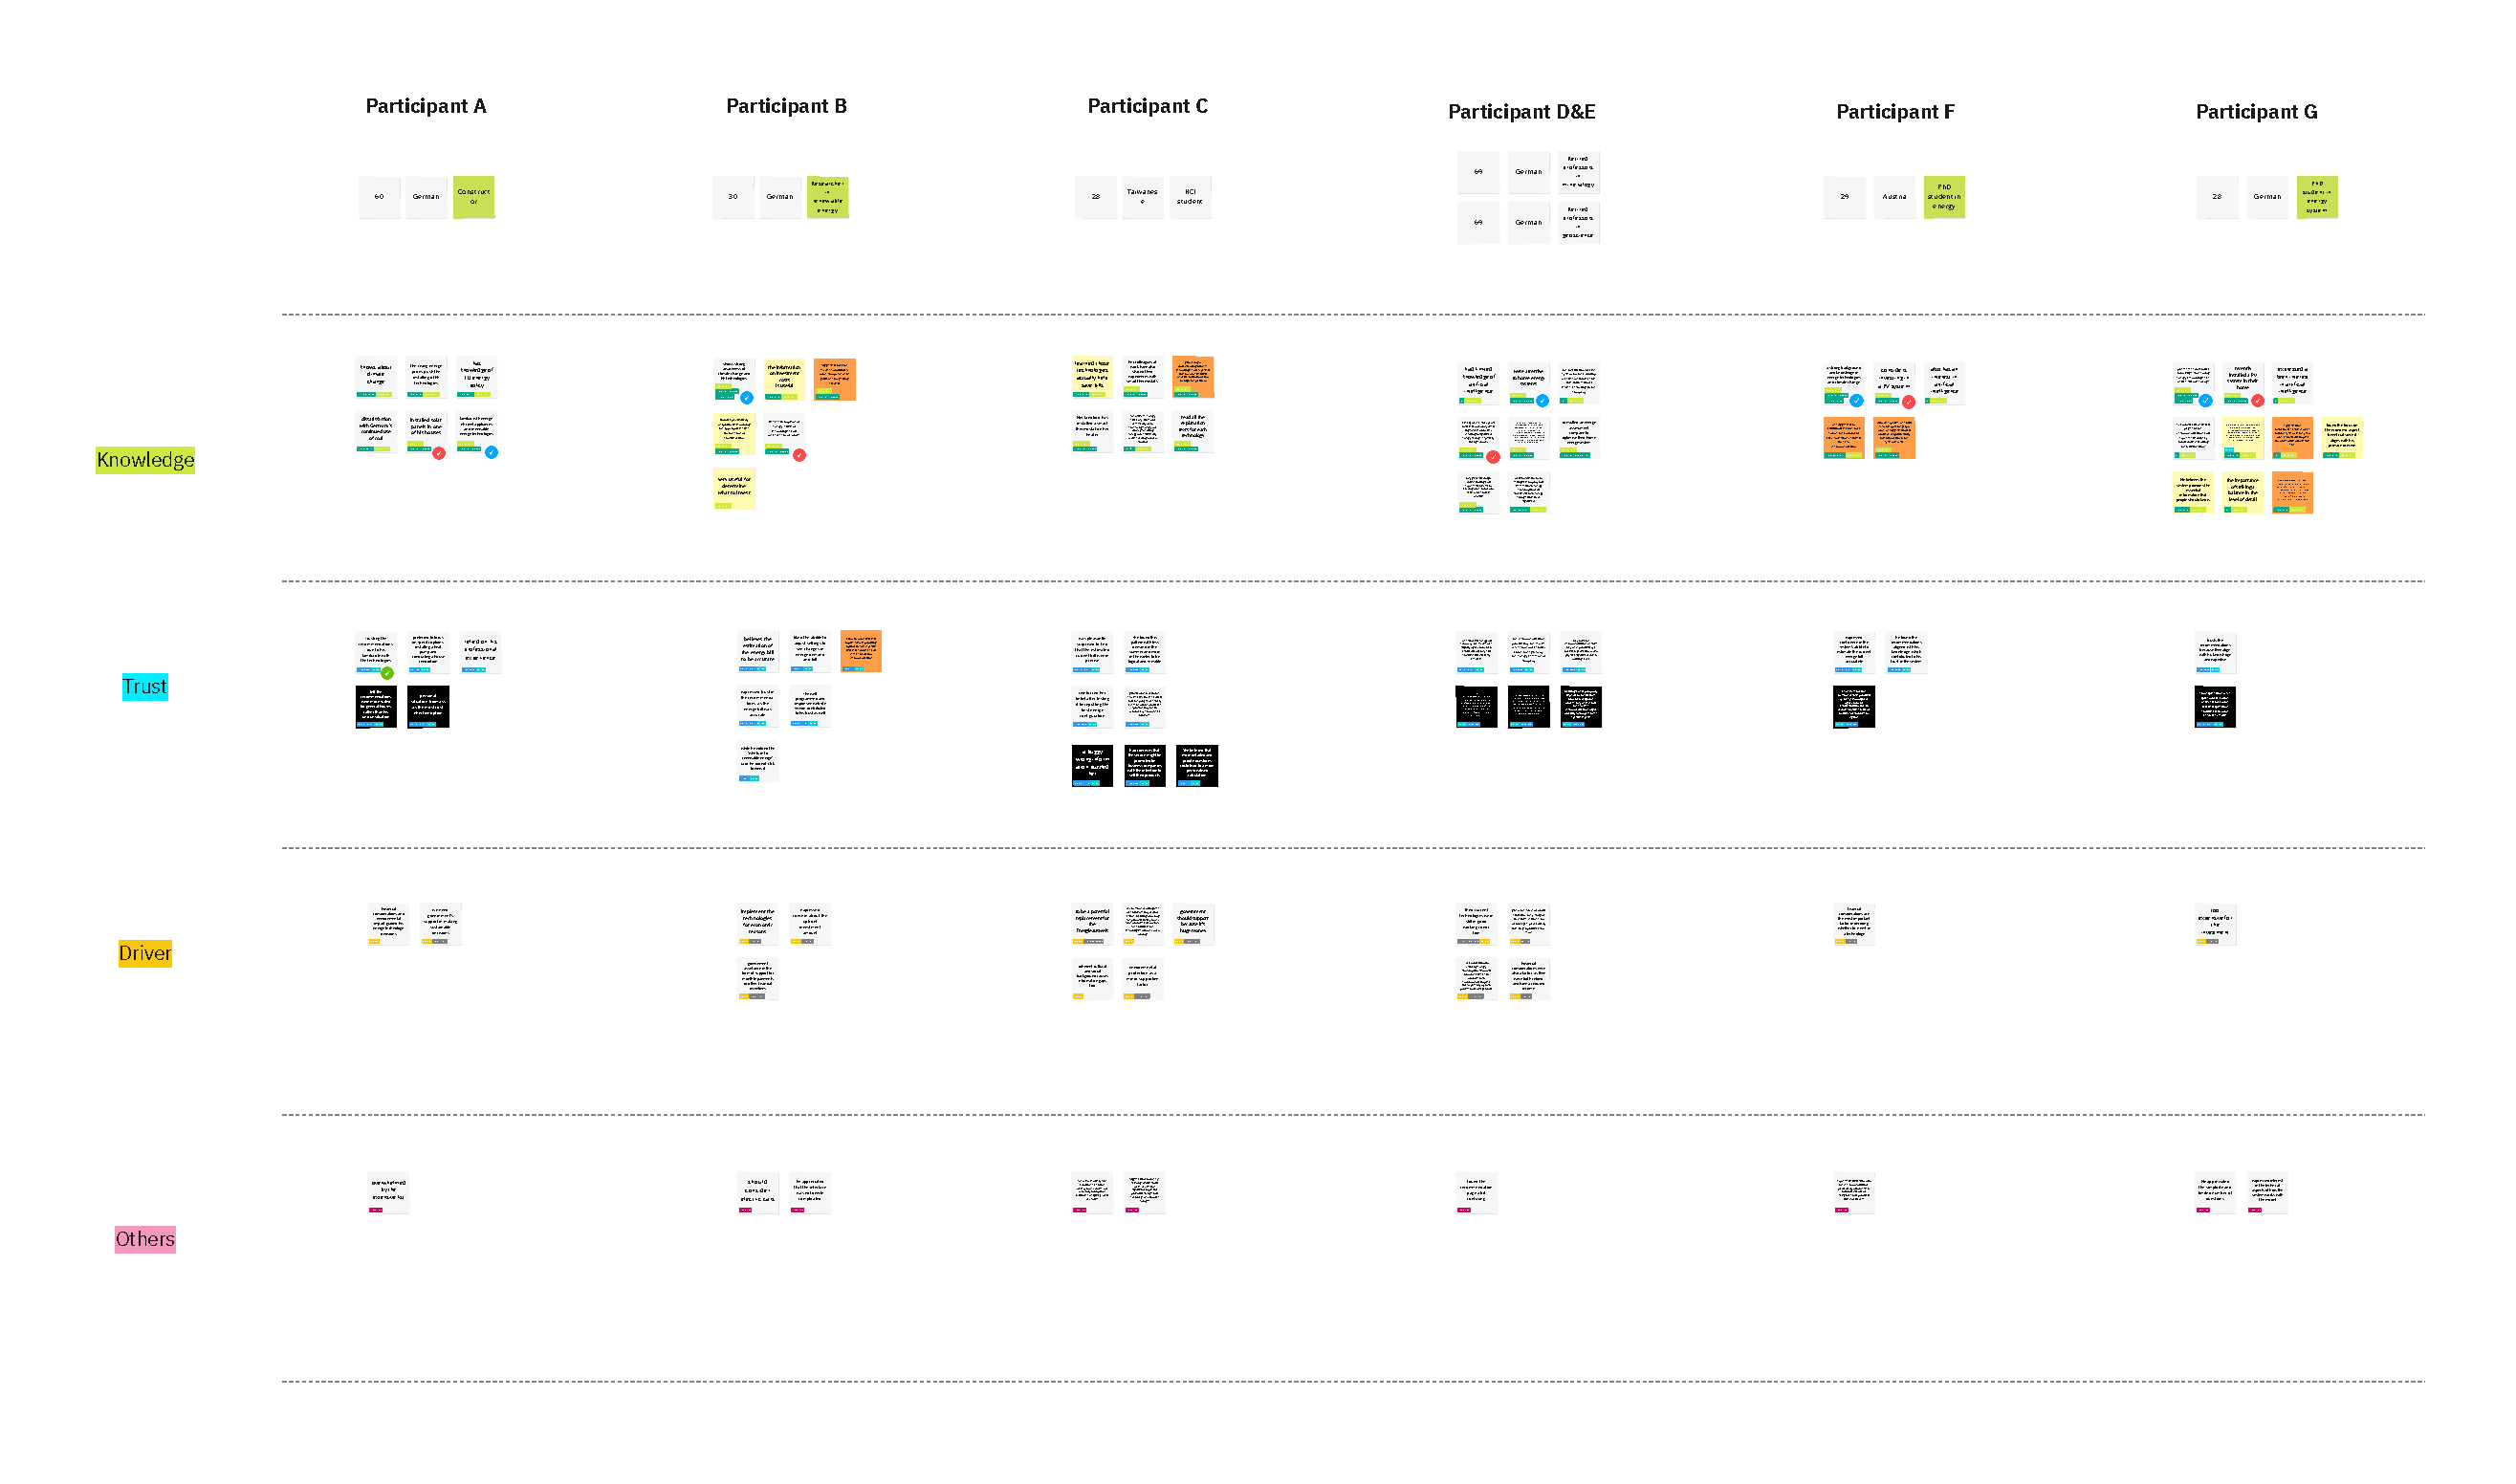
\includegraphics[width=\textwidth]{Images/thematic.pdf}
  \caption{Thematic analysis}
  \label{fig:thematic}
\end{figure}

Figure \ref{fig:thematic1}, Figure \ref{fig:thematic2}, Figure \ref{fig:thematic3}, and Figure \ref{fig:thematic4} display the categorised clusters of sticky notes for each respective topic.
\begin{figure}[h!]
  \centering
  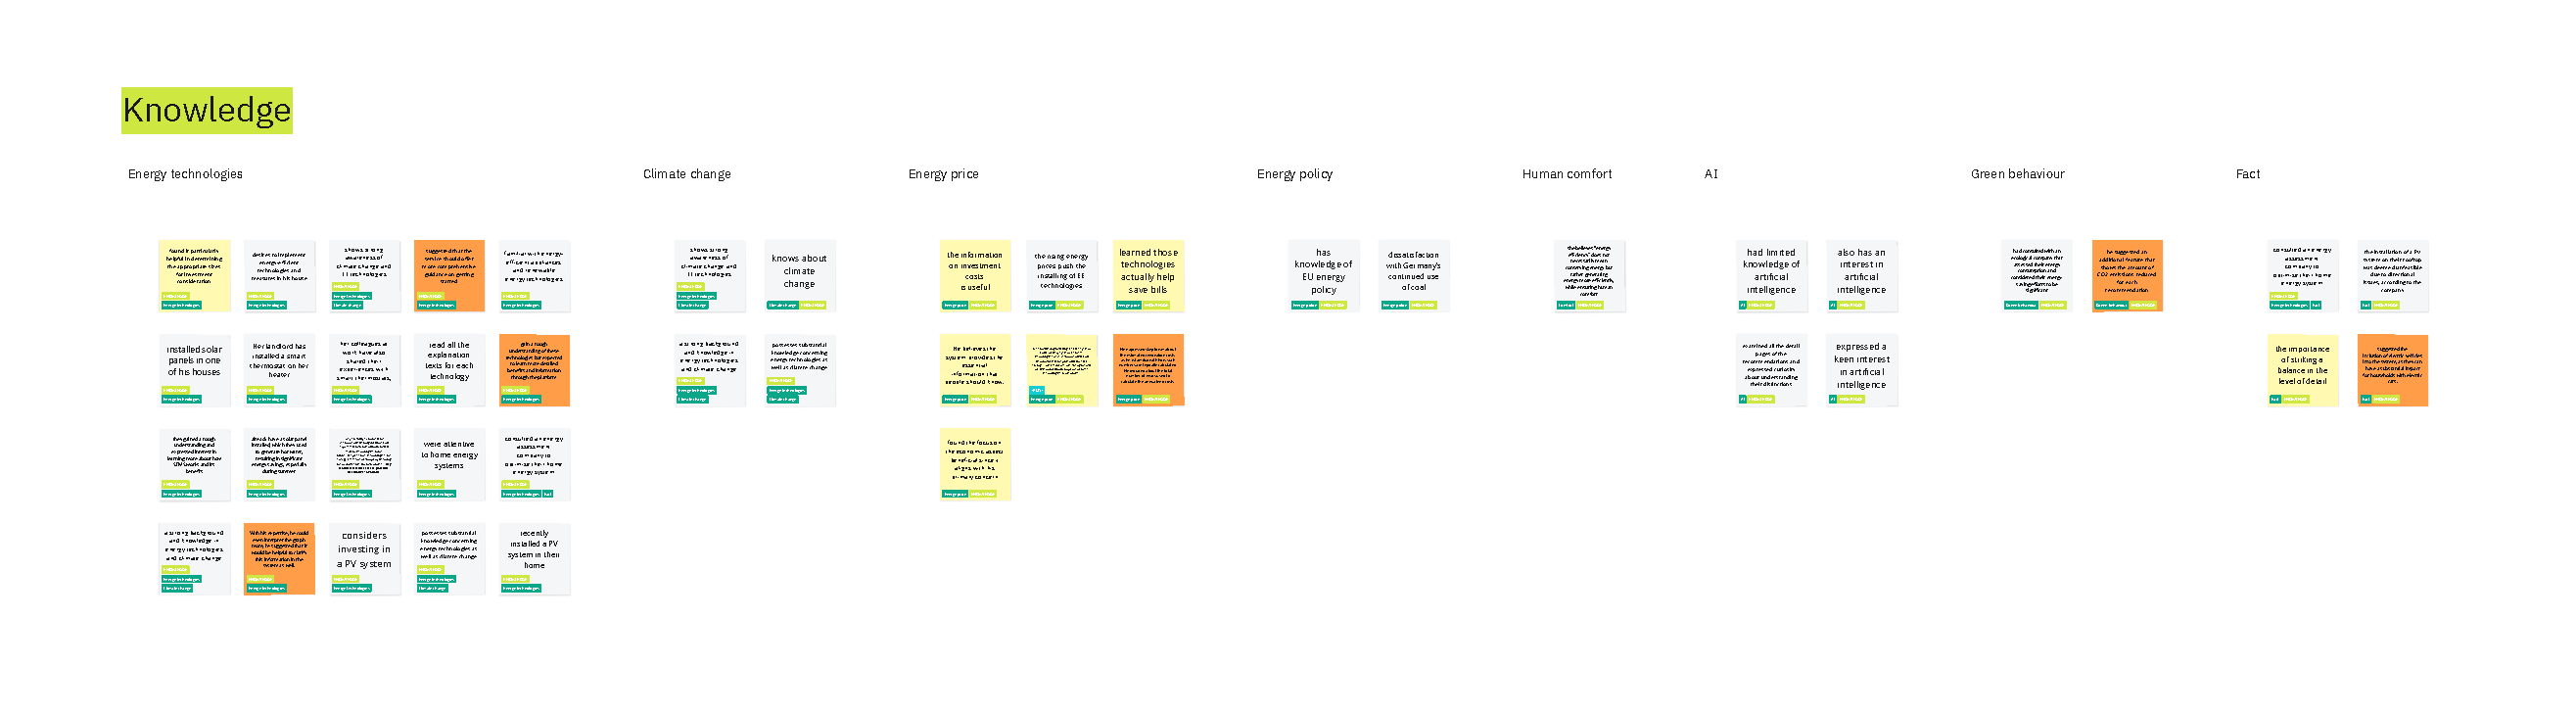
\includegraphics[width=\textwidth]{Images/thematic1.pdf}
  \caption{Thematic analysis: Knowledge}
  \label{fig:thematic1}
\end{figure}
\begin{figure}[h!]
  \centering
  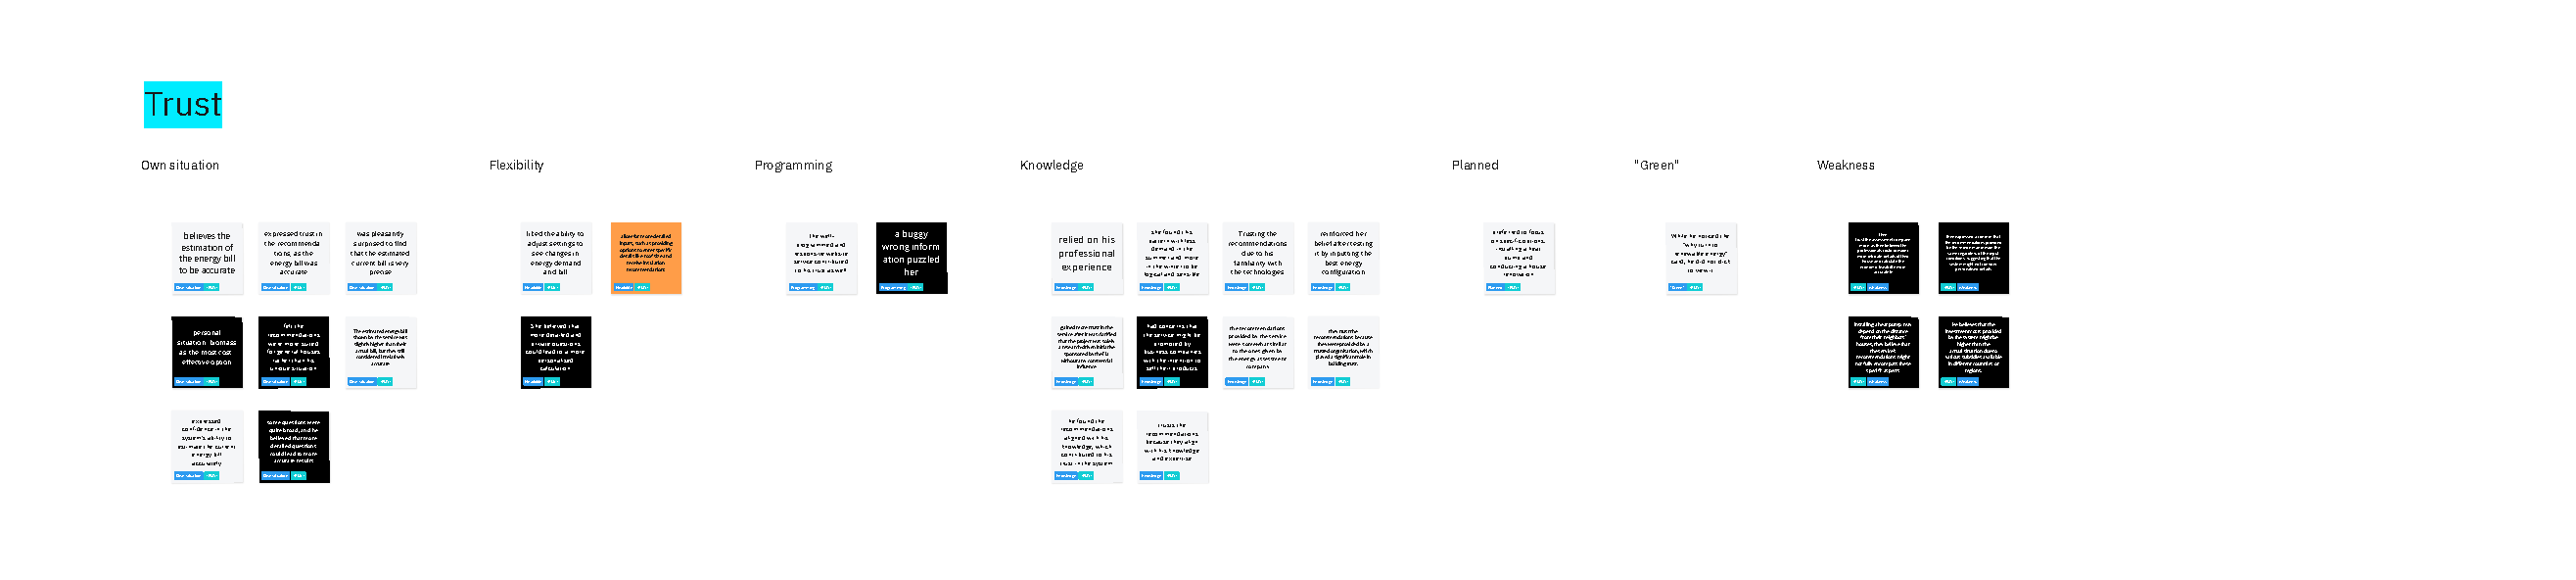
\includegraphics[width=\textwidth]{Images/thematic2.pdf}
  \caption{Thematic analysis: Trust}
  \label{fig:thematic2}
\end{figure}
\begin{figure}[h!]
  \centering
  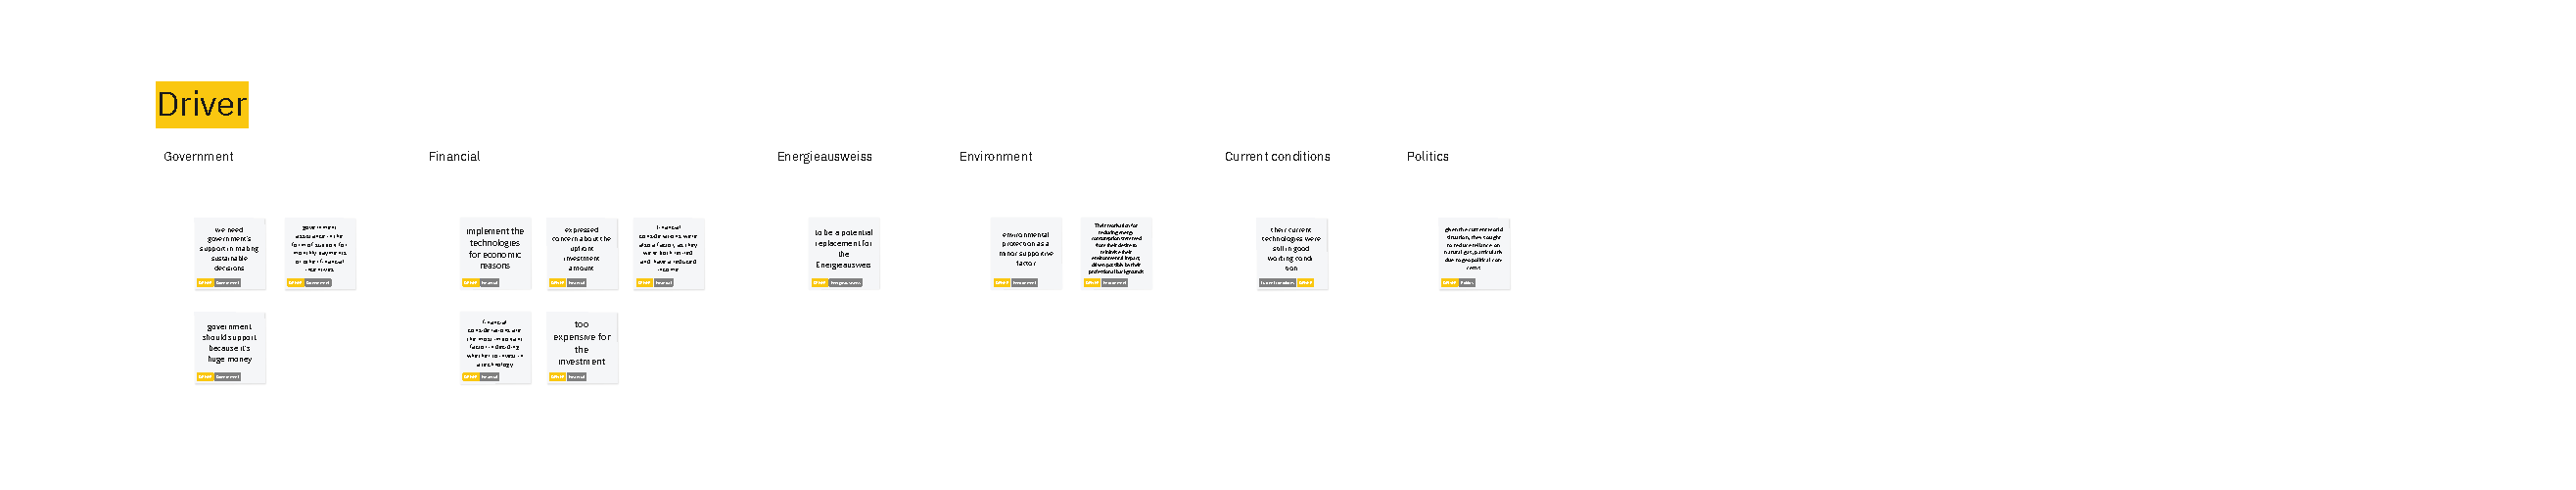
\includegraphics[width=\textwidth]{Images/thematic3.pdf}
  \caption{Thematic analysis: Driver}
  \label{fig:thematic3}
\end{figure}
\begin{figure}[h!]
  \centering
  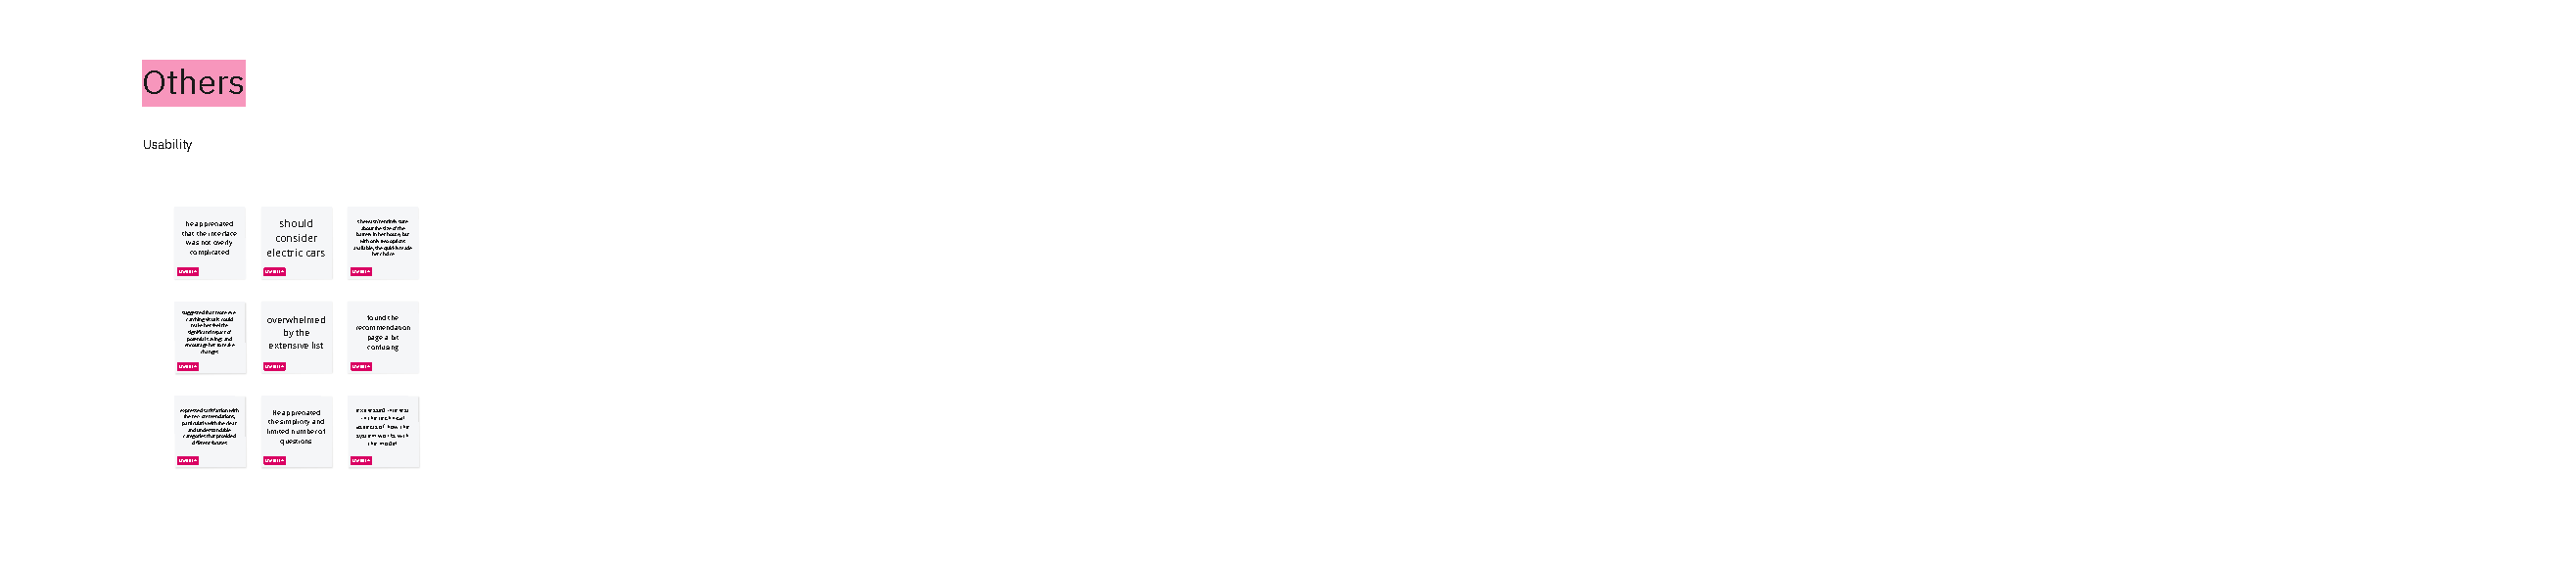
\includegraphics[width=\textwidth]{Images/thematic4.pdf}
  \caption{Thematic analysis: Other}
  \label{fig:thematic4}
\end{figure}


Table \ref{tab:participants_perceptions} provides an overview of participants' general understanding and interest in artificial intelligence and energy technologies, 
along with their perspectives on the service's learnability and explainability. 
\begin{table}[h!]
  \centering
  \begin{tabular}{ | p{.10\textwidth} | p{.15\textwidth} | p{.15\textwidth} | p{.15\textwidth} | p{.15\textwidth} | } 
    \hline
    ID & Interest in AI & Interest in energy & Learned more & Trust \\
    \hline
    PA & No & Yes & No & Yes \\
    \hline
    PB & No & Yes & Yes & Yes \\
    \hline
    PC & No & No & Yes & Not much \\
    \hline
    PD & No & Yes & Yes & Yes \\
    \hline
    PE & No & Yes & Yes & Yes \\
    \hline
    PF & Yes & Yes & No & Yes \\
    \hline
    PG & Yes & Yes & No & Yes \\
    \hline
  \end{tabular}
  \caption{Participants' understanding and perspectives}
  \label{tab:participants_perceptions}
\end{table}

Moreover, the complete interview transcripts are available in Appendix \ref{appendix:transcription}.


\subsubsection{Participant A}

Before using the service, 
Participant A, who works in the house construction industry, 
displayed knowledge of EU energy policy and familiarity with energy-efficient appliances and renewable energy technologies. 
He had implemented solar panels in one of his houses and believed in their ability to reduce energy costs for households. 
Participant A emphasised the rising energy prices and the importance of addressing climate change, expressing dissatisfaction with Germany's continued use of coal. 

During the service usage, 
Participant A found the service to work smoothly, receiving a comprehensive list of around 50 recommendations to lower energy costs. 
While he agreed with most configurations, he felt overwhelmed by the extensive list and preferred to focus on specific options such as installing a heat pump and conducting a house renovation, given his expertise in his own house's needs. 
Despite not finding recommendations for biomass utilisation, Participant A relied on his professional experience and personal resources in considering biomass as the most cost-effective option. 
Although he missed the last level of explanation on renewable energy benefits, he clicked to view more details on the specific recommendation he sought.

After using the service, 
Participant A appreciated the recommendations but felt they were more suited for general houses rather than his unique situation. 
Financial considerations and environmental impact guided his energy technology decisions. 
Trusting the recommendations due to his familiarity with them, he acknowledged the service provided an overwhelming amount of information and a surplus of recommendations.


\subsubsection{Participant B}

Before using the service, 
Participant B, who works in the renewable energy industry, 
expressed a strong awareness of climate change and a desire to implement energy-efficient technologies and measures in his house primarily for economic reasons.

During the service usage, 
Participant B found the service to be simple, clean, and straightforward, which he appreciated. 
Although the service did not consider his electric car, he believed the estimation of the remaining energy bill to be accurate. 
He found the information on investment costs to be useful and liked the ability to adjust settings to see changes in energy demand and bill. 
While he noticed the "why turn to renewable energy" card, he did not click to view it.

After using the service, 
Participant B found it particularly helpful in determining the appropriate sizes for investment consideration. 
He believed that implementing these technologies could lead to energy cost savings, 
but expressed concern about the upfront investment amount, which posed a barrier for him. 
He suggested that government assistance in the form of support for monthly payments or other financial incentives could make green living more accessible. 
Participant B also suggested that the service should offer more comprehensive guidance on getting started 
and allow for more detailed inputs, such as providing options to enter specific details like roof size and receive insulation recommendations. 
He expressed trust in the recommendations, as the energy bill was accurate when not considering the electric car. 
The well-programmed and responsive website service contributed to his trust as well, and he appreciated that the interface was not overly complicated.


\subsubsection{Participant C}

Before using the service, 
Participant C, a current master's student in human-computer interaction, 
admitted that she doesn't have much knowledge or interest in artificial intelligence, nor energy technologies. 
She does have a smart thermostat installed on her heater, which was provided by her landlord, and she is familiar with how it operates. 
Additionally, her colleagues at work have also shared their experiences with smart thermostats, as many of them have one. 
She holds the belief that the concept of ``energy efficiency" does not necessarily mean conserving energy but rather generating energy more efficiently, while ensuring human comfort.

During the service usage, 
Participant C carefully read all the explanation texts for each technology while providing the current configuration of her house. 
She wanted to ensure that she answered correctly. 
When selecting the battery capacity, she wasn't entirely sure about the size of the battery in her house, but with only two options available, she quickly made her choice, believing that the battery in her house should be a larger one.
After receiving the estimates of her current annual energy bill, Participant C calculated the monthly bill herself and was pleasantly surprised to find that it was very precise. 
She then proceeded to choose a recommendation and closely examined the accompanying energy graphs. 
Noticing that the energy demand bars for each month showed variations, with less demand in the summer and more in the winter, she found this pattern to be logical and sensible.
However, she also encountered a confusing aspect when she noticed an energy bar for cooling, even though she didn't have an air conditioner in her house. This information puzzled her. 
Participant C also clicked on the climate change education card to quickly scan its content and appreciated the information being presented in that section.

After using the service, 
Participant C found it to be a potential replacement for the Energieausweis, a nation-wide recognised standard in Germany for displaying a house's energy-efficiency level, which people usually need to pay professionals for. 
She appreciated that the recommendations were presented in a neutral manner, 
but suggested that more eye-catching visuals could make her feel the significant impact of potential savings and encourage her to make changes.

Participant C felt that the recommendations might not perfectly align with her own situation,
because the questions asked in terms of her energy consumption behaviours, were relatively general. 
She believed that more detailed and private questions could lead to a more personalised calculation. 
Regarding trust, she initially believed in the service, 
especially after seeing that the estimated energy bill was accurate. 
However, when she encountered confusion in the graph, her trust in the system wavered. 
Participant C had concerns that the service might be promoted by business companies with the intention to sell their products. 
This led her to believe that the algorithm behind the model might be biased and pushing users to spend money. 
However, after it was clarified that the project was solely a research-driven initiative sponsored by the EU without any commercial influence, she gained more trust in the service.
To further validate her trust in the system, she decided to test it by inputting the best energy configuration. 
The service did not provide any recommendation for this situation, which reinforced her belief that the system was not solely focused on pushing users to spend money. 
This positive experience increased her trust in the service and the recommendations. 

Participant C also mentioned that her investment willingness was influenced by various factors, 
including how long she planned to stay in her current house and whether she could take the technologies with her when moving. 
In her background, households were not allowed to privately install \gls{pv} systems without obtaining a certificate from authorities, 
and selling excess electricity back to the grid was prohibited. 
which differs from Europe where governments encourage \gls{pv} installations. 
Upon learning about these differences, she became enthusiastic about installing a PV system, 
recognising its benefits in both cost savings and contributing to environmental preservation.

Despite not having much prior knowledge of energy technologies, 
Participant C was able to answer all questions about her current house after reading the descriptions provided. 
She mentioned that the service allowed her to gain a rough understanding of these technologies but expected to learn more detailed benefits and information through the platform.


\subsubsection{Participant D \& E}

Before using the service, 
Participant D and Participant E, a couple, 
had limited knowledge of artificial intelligence but were attentive to home energy systems. 
They already had a solar panel installed, which they used to generate hot water, resulting in significant energy savings, especially during summer. 
Seven years ago, they consulted an energy assessment company to optimise their home energy system. 
The company assessed the feasibility of installing various technologies and provided suggestions. 
Notably, the installation of a \gls{pv} system on their rooftop was deemed unfeasible due to directional issues, according to the company.

While they wished to transition to more energy-efficient technologies eventually, 
some of their current technologies were still in good working condition. 
They planned to replace them in the future when they no longer served efficiently. 
Their motivation for reducing energy consumption stemmed from their desire to minimise their environmental impact, 
driven possibly by their professional backgrounds. 
Moreover, given the current world situation, they sought to reduce reliance on natural gas, 
particularly due to geopolitical concerns, as they preferred not to buy gas from Russia. 
Financial considerations were also a factor, as they were both retired and have a reduced income.

During the service usage, 
Participant D and Participant E found the recommendation page a bit confusing, but they understood it better after I explained the page. 
The estimated energy bill shown by the service was slightly higher than their actual bill, but they still considered it relatively accurate. 
They carefully examined the recommended configurations and expressed their intention to install certain technologies in the future, 
despite some technologies, the energy assessment company deeming them unfeasible for their house. 
They wondered if there were portable alternatives available. 
Additionally, they were unfamiliar with the \gls{sems} system, but after reading the provided explanation, they gained a rough understanding and expressed interest in learning more about how it works and its benefits.
They found the energy visualisation feature interesting and, with my guidance, explored the additional information on climate change and energy-saving measures for individuals.
They briefly read through the information and agreed with the suggested measures, mentioning that they already follow some of those practices. 
They also shared that they had consulted with an ecological company that assessed their energy consumption and considered their energy-saving efforts to be significant. 
In an effort to be more energy-efficient, they even turned down the temperature a bit, and dress more in the house. 

After using the service, 
Participant D and Participant E noted that the recommendations provided by the service were somewhat similar to the ones given by the energy assessment company.
However, they highlighted that the energy assessment company provided more personalised suggestions as they physically visited their house and could offer more precise advice tailored to their specific situation. 
Despite this, they expressed trust in the service's recommendations, particularly because they were provided by a trusted organisation, which played a significant role in building trust.
However, they trust the assessment company more, as they believed the professionals could consider more intricate details of their house and calculate the economic feasibility more accurately. 
Since Participant D and Participant E live in a house with shared walls with neighbors, they emphasised that several additional factors should be considered when installing new technologies. 
For example, changes to insulation on the rooftop or walls and the feasibility of installing a heat pump may depend on the distance from their neighbors' houses. 
Consequently, they believe that the service's recommendations might not fully encompass these specific aspects. 
Furthermore, they expressed a concern that the recommendations provided by the service may remain the same regardless of the input conditions, suggesting that the system might not consider personalised details. 
This led to a slight skepticism regarding the variability and suitability of the recommendations under different circumstances.


\subsubsection{Participant F}

Before using the service, 
Participant F is pursuing a PhD degree in the energy domain, indicating a strong background and knowledge in energy technologies and climate change. 
Additionally, Participant F also has an interest in artificial intelligence.

During the service usage, 
Participant F found the experience to be smooth and had no difficulties receiving the recommendations. 
He expressed confidence in the system's ability to estimate the current energy bill accurately. 
Despite all the recommendations suggesting investments that would not yield cost benefits (i.e., the annualised investments exceed potential savings on energy bills), 
Participant F still considers investing in a \gls{pv} system. 
He believes that the investment costs provided by the system might be higher than the actual situation due to various subsidies available in different countries or regions, which could potentially reduce the overall investment.
While Participant F appreciated the bar charts displaying electricity demand and generation, 
he suggested an additional feature that shows the amount of \gls{co2} emissions reduced for each recommendation. 
He believes that such a feature would allow for a more contrasting comparison, 
as the electricity consumption alone may not clearly indicate the environmental impact. 
He mentioned that when some recommendations show higher estimates than the previous ones, 
having this \gls{co2} reduction information could provide a more obvious indication of their positive impact.

After using the service, 
Participant F expressed satisfaction with the recommendations, particularly with the clear and understandable categories that provided different focuses. 
He trusted the recommendations and the estimations of energy consumption. 
Besides the investment costs provided by the system might be higher than the actual costs due to potential subsidies not considered in different areas, 
especially when it comes to investing in a \gls{pv} system.
For Participant F, financial considerations are the most important factor in deciding whether to invest in a technology. 
As someone working in the related field, he found the recommendations aligned with his knowledge, which contributed to his trust in the system. 
With his expertise, he could even interpret the graph to determine how much hot water was heated by the \gls{pv} system and how much was produced by the boiler. 
He suggested that it would be helpful to clarify this information in the system as well. 


\subsubsection{Participant G}

Before using the service, 
Participant G is a researcher specialising in energy systems, 
and thus, he possesses substantial knowledge concerning energy technologies as well as cliamte change. 
He also expressed a keen interest in artificial intelligence. 
Participant G lives with his family and recently installed a \gls{pv} system in their home.

During the service usage, 
Participant G navigated through all the questions effortlessly and successfully received all three recommendations. 
He appreciated the simplicity and limited number of questions, 
although he is able to provide more detailed answers. 
However, he considered that regular homeowners might not be able to answer more intricate questions. 
Participant G carefully examined all the detail pages of the recommendations and expressed curiosity about understanding their distinctions.

After using the service, 
Participant G found the focus on the economic aspect beneficial since it aligns with his primary concern. 
He and his family are considering installing a \gls{sems} system and a battery system, 
as these technologies were recommended and demonstrated the potential for cost savings. 
This assurance has strengthened his determination to implement these technologies in his house. 
He believes the system provides the essential information that people should know. 

One concern raised by Participant G was related to house renovation costs, 
as he considered them too expensive for the investment. 
He expressed skepticism about the estimated renovation costs, 
as he is familiar with how such numbers are typically calculated. 
He inquired about the total number of years used to calculate the annualised costs.
Participant G suggested the inclusion of electric vehicles into the system, 
as they can have a substantial impact for households with electric cars. 

Being well-versed in the energy sector, he has a great understanding of how electricity is managed. 
In fact, he could even explain the energy demand and generation graphs based on his expertise.
Overall, Participant G trusts the recommendations because they align with his knowledge and expertise. 
However, he pointed out that some questions were quite broad, and he believed that more detailed questions could lead to more accurate results. 
Nonetheless, he acknowledged the importance of striking a balance in the level of detail.

In the end, Participant G expressed interest in the technical aspects of how the system works with the model. 


\section{Discussion}

As per the participants' feedback, 
all of them show a strong awareness of climate change. 
Four of the participants, who work in energy-related fields, have significant knowledge about energy technologies due to their job experiences. 
Two participants gained their knowledge from consulting experts in the field. 
Only one participant had limited familiarity with energy technologies. 
Furthermore, all participants, except this one, have either already installed or are planning to install energy-efficient technologies in their homes. 
This is likely because individuals who are already interested in energy topics are more inclined to take part in this kind of research.


\subsection{Participants lack of knowledge wish to learn more}

In terms of energy technologies, participants who already had some knowledge didn't significantly enhance their understanding through the service. 
Only two participants, who were unfamiliar with \gls{sems}, learned about this specific technology. 
Together with the one participant with limited prior knowledge appreciated the general overview provided by the service but found it lacking in depth. 
They expressed a desire for more detailed information on the technologies. 
It seems that offering only basic explanations isn't sufficient. 
There's a need to provide additional detailed information for users keen on expanding their knowledge about these technologies.


\subsection{Financial considerations drive decisions}

All participants emphasised the critical role of the financial aspect when making decisions about energy technology investments. 
As stated by one participants, 
\begin{displayquote}
  ``The focus on the economic aspect is beneficial since it is my primary concern.''. 
\end{displayquote}
This sentiment was reinforced by a participant from the construction field, who highlighted the impact of rising fuel and gas prices as a driving force behind people's shift towards renewable energy due to its cost-effectiveness.

One participant mentioned the information on investment costs is crucial, helping him make informed decisions. 
Moreover, the estimated energy bills were deemed valuable for determining the technology choices and sizes, as another participant explained.
Furthermore, one participant's preferred technologies were recommended by the service, leading to increased confidence in the investment due to the estimated bill reductions.

The participant with limited knowledge of energy technologies recognised the potential for significant cost savings through the service, 
this feedback shows the significance of maintaining an emphasis on financial aspects within the service, 
showcasing its potential to bridge the information gap in this vital area. 
The focus on financial considerations not only aligns with participants' primary concerns but also serves as a key driver in encouraging sustainable energy choices.


\subsection{Energy professionals seeking in-depth information}

In our evaluation, all three participants with expertise in the energy sector shared a common request for more comprehensive information regarding the recommendations provided. 
They demonstrated a strong ability to interpret the visualised charts depicting energy demand and generation.
Moreover, they are interested into the technical intricacies of the model or algorithms. 

One participant expressed interest in having the reduction amount of \gls{co2} emissions displayed for each recommendation. 
This participant believed that this information would present more obvious differences than the energy charts, 
and also providing a clearer understanding of the environmental impact of different choices.
Another participant indicated a desire to understand how the renovation costs were calculated. 
The feedback from participants with professional energy knowledge underscores their inclination towards acquiring more comprehensive details of the model, 
revealing their pursuit of in-depth explanations and a desire to make informed decisions based on these insights. 
They request greater transparency in the system's underlying processes.


\subsection{Solid trust across participants}

In our evaluation, all participants expressed trust in the recommendations provided by the system. 
This trust was fortified by several factors, each playing a role in building their confidence.


\subsubsection{Accurate energy bill estimations build credibility}

Mentioned by all participants,
a significant contributor to this trust is the perceived accuracy of the estimated current energy bills. 
Participants' conviction in the correctness of these estimates was instrumental in fostering trust in the recommendations.


\subsubsection{Professional expertise bolsters trust}

Participants engaged in energy-related fields resonated with the recommendations due to their alignment with their professional knowledge. 
This correspondence between the system's suggestions and their expertise augmented their trust in the system's advice.


\subsubsection{Trusted source and research institution}

For some participants (3 out of 7), the fact that the service was developed by a trusted organisation was a significant trust-building factor.
This is evidenced by one example, one participant initially had doubts, fearing that the service might be influenced by business interests promoting specific energy technologies. 
However, these concerns diminished as the participant noticed that certain configurations received no recommendations, revealing the service's impartiality. 
His trust solidified upon learning that the service was crafted by a research institute rather than a commercial entity. 
Therefore, the importance of transparently conveying the intention to users is evident. 


\subsubsection{Consistency with past recommendations reinforces confidence}

Two participants who had prior experience with energy audits found the recommendations from the service to be consistent with those obtained elsewhere. 
This alignment reinforced their confidence in the service's recommendations.


\subsubsection{Design and user experience boosters confidence}

Another participant highlighted the role of the well-designed, responsive web interface in building trust. 
A user-friendly interface contributes to a sense of professionalism and reliability, further strengthening trust in the system.


\subsection{Personalisation concerns}

The feedback received also highlighted concerns regarding the level of personalisation in the recommendations. 
Notably, participants underlined situations where their unique circumstances weren't fully accounted for.


\subsubsection{Unique resources situations}

Among the participants, some (2/7) presented unique circumstances. 
A participant, who works in the house construction field, believed that his house's situation differed from typical households. 
This participant emphasised that a biomass boiler was a more economical solution for him.
His house had ample space for wood storage due to a large garden, and his proximity to forests meant that biomass prices were lower for him. 
A similar sentiment was echoed by another participant who couldn't install a \gls{pv} system due to specific directional constraints of their house. 
This information was informed by professionals during an energy audit.


\subsubsection{Unique consumption behaviours}

Another participant mentioned that the service didn't delve into his specific energy consumption behaviours. 
He believed his energy usage differed from the norm, which might impact the accuracy of the estimations. 
Similarly, another participant expressed concerns, suggesting that certain questions in the service could be more detailed. 
This participant believed that greater detail in the questions could lead to more accurate calculations and recommendations. 
These observations underscore the need to strike a balance between simplicity and detail in the questions presented to users. 


\subsubsection{Regional variations in investment costs}

From a financial perspective, one participant brought up the point that investment costs could fluctuate based on regional differences. 
This is due to varying subsidy policies that are often tied to specific geographical areas.


\subsubsection{Beyond technologies}

In addition to the focus on energy technologies and their sizes, few participants (2/7) expressed a desire for more granular and comprehensive recommendations. 
One participant expressed an interest in receiving recommendations for the materials to be employed in rooftop renovations. 
Another participant expressed a need for greater clarification on how to initiate changes in their energy system. 
These insights emphasise the significance of considering users' holistic needs and expanding the scope of recommendations to encompass various aspects of energy-efficient enhancements to ensure a more comprehensive and user-centric approach, catering to a diverse range of user preferences and requirements.


\subsection{Motivations for investment: financial and beyond}

The driving force behind participants' motivation to invest in energy-efficient technologies predominantly revolves around financial considerations. 
The allure of potential cost savings on energy bills appears to be the primary incentive for most participants. 
Additionally, environmental protection emerges as a notable supporting factor in participants' decision-making. 
While financial benefits are at the forefront, the desire to contribute positively to the environment underscores a collective recognition of the importance of sustainable energy practices.
It's noteworthy that nowadays geopolitical concerns also play a role for a subset of participants. 


\subsection{Government Support}

In terms of financial implications, the participants shared a consensus that investing in a sustainable energy system involves substantial financial commitment. 
This sentiment echoes the general understanding that adopting energy-efficient technologies often requires a significant upfront investment.
A substantial portion of the participants (3/7) expressed the view that government support should play a pivotal role in facilitating the adoption of sustainable energy systems.
This insight emphasises the role of governments in incentivising and promoting the adoption of energy-efficient technologies, potentially through subsidies, tax benefits, or other forms of financial assistance. 


\subsection{A multifunctional perspective}

An intriguing perspective arose from one participant, shedding light on the multifunctional potential of the service. 
Beyond its primary role of offering energy system recommendations, this participant recognised the service as a potential alternative to the commonly required "Energieausweis" (energy certificate) \cite{verbraucherzentrale} in certain regions. 
This certificate is a significant document used to assess a property's energy efficiency, typically mandated for property transactions and rentals.
Such multifunctionality adds a layer of versatility to the service, potentially expanding its reach and relevance within the energy domain.